\documentclass[10pt,a4paper]{report}
\usepackage[utf8]{inputenc}
\usepackage[portuguese]{babel}
\usepackage[T1]{fontenc}
\usepackage{amsmath}
\usepackage{lmodern}
\usepackage{amsfonts}
\usepackage{amssymb}
\usepackage{graphicx}
\title{\Huge{Introduç\~ao às Probabilidades e Estatística} \\ \vspace{1cm}
       \huge{Resumo}}
\author{\large {Jo\~ao Matos}}
\date{}
\begin{document}

\maketitle

\chapter{Probabilidade}

\section{Massa de probabilidade (variáveis discretas)}

\subsection{Modelo Binomial}
É a distribuição do número de sucessos obtidos depois de $n$ ensaios de Bernoulli independentes de parâmetros $p\in [0,1]$, ou seja, é a distribuição da soma de $n$ variáveis aleatórias independentes da distribuição de Bernoulli de mesmo parâmetro.
O modelo binomial é utilizado quando se verificam as seguintes propriedades:
\begin{itemize}
\item Cada tentativa tem exclusivamente como resultado duas possibilidades, sucesso ou fracasso;
\item Cada tentativa é independente das demais;
\item A probabilidade de sucesso $p$ a cada tentativa permanece constante independente das demais;
\item A variável de interesse, ou pretendida, é o número de sucessos $k$ nas $n$ tentativas.
\end{itemize}

As suas variáveis aleatórias s\~ao dadas por:\\

$$
X \cap B(n, p)
$$

E a sua f.m.p é dada por:\\

$$
P(X = k) = \begin{pmatrix}
n \\
k
\end{pmatrix} p^k(1-p)^{n-k}, k = 0, 1, 2, ..., n
$$

\vspace{0.7cm}

O seu valor médio é $E(X)=np$ e a variância é $var(X)=np(1-p)$

\vspace{0.7cm}

A soma de variáveis aleatórias independentes com distribuiç\~ao binomial  é calculada como:

$$
\sum_{i=1}^{n} X_i \cap B\left(\sum_{i=1}^{n} n_i, p\right)
$$

\subsection{Modelo Geométrico}
É a distribuição que modela o tempo de espera do primeiro sucesso de uma de ensaios de Bernoulli independentes com probabilidade de sucesso $ p\in [0,1]$. É a única distribuição discreta que possui a propriedade de falta de memória.\\
As suas variáveis aleatórias s\~ao dadas por:\\

$$
X \cap G(p)
$$

E a sua f.m.p é dada por:\\

$$
P(X = k) = (1-p)^{k-1}p, k = 1, 2,...
$$

\vspace{0.7cm}

O seu valor médio é $E(X)=\frac{1}{p}$ e a variância é $var(X)=\frac{1-p}{p^2}$


\subsection{Modelo Binomial Negativo}
Esta distribuição indica o número de tentativas necessárias para obter $r$ sucessos de igual probabilidade $p$ ao fim de n experimentos de Bernoulli, sendo a última tentativa um sucesso.
As suas variáveis aleatórias s\~ao dadas por:\\

$$
X \cap BN(r, p)
$$

E a sua f.m.p é dada por:\\

$$
P(X = k) = \begin{pmatrix}
k-1 \\
r-1
\end{pmatrix} p^r(1-p)^{k-r}, k = r, r+1, ...
$$

\vspace{0.7cm}

O seu valor médio é $E(X)=\frac{r}{p}$ e a variância é $var(X)=\frac{r(1-p)}{p^2}$

\subsection{Modelo Hipergeométrico}
A distribuição hipergeométrica modela uma retirada simultânea de $n$ bolas uma urna contendo uma proporção $pN$ de bolas vencedoras e uma proporção $(1-p)N$ de bolas perdedoras para um número total $N$ de bolas. A distribuição descreve o número de bolas vencedoras extraídas.

As suas variáveis aleatórias s\~ao dadas por:\\

$$
X \cap H(N, n, p)
$$

E a sua f.m.p é dada por:\\

$$
P(X = k) = \frac{\begin{pmatrix}
M\\
k
\end{pmatrix}\begin{pmatrix}
N-M\\
n-k
\end{pmatrix}}{\begin{pmatrix}
N\\
M
\end{pmatrix}}
, k = max(0, n-(N-M)),..., min(M,n)
$$

\vspace{0.7cm}

O seu valor médio é $E(X)=np$ e a variância é $var(X)=np(1-p)\frac{N-n}{N-1}$

\subsection{Modelo de Poisson}
A distribuição de Poisson descreve o comportamento do número de eventos que ocorrem em um espaço determinado de tempo.

As suas variáveis aleatórias s\~ao dadas por:\\

$$
X \cap P(\lambda)
$$

E a sua f.m.p é dada por:\\

$$
P(X = k) = e^{-\lambda}\frac{\lambda^k}{k!}
, k = 0, 1, 2, ... \hspace{0.5cm} (\lambda > 0)
$$

\vspace{0.7cm}

O seu valor médio é $E(X)=\lambda$ e a variância é $var(X)=\lambda$

\vspace{0.7cm}

A soma de variáveis aleatórias independentes com distribuiç\~ao de Poisson  é calculada como:

$$
\sum_{i=1}^{n} X_i \cap P\left(\sum_{i=1}^{n} \lambda_i\right)
$$

\section{Distribuiç\~ao (variáveis contínuas)}

\subsection{Modelo Uniforme}
A distribuiç\~ao uniforme corresponde á a probabilidade de se gerar qualquer ponto num intervalo contido no espaço amostral que é proporcional ao tamanho do intervalo, visto que na distribuição uniforme a $f(x)$ é igual para qualquer valor de x no intervalo considerado. Por exemplo, se considerarmos um intervalo em x de zero à dez, $(x \in [0,10])$, e assumirmos que temos uma distribuição uniforme nesse intervalo, a probabilidade de f(x) no intervalo  2<x<5 é igual a probabilidade de f(x) no intervalo  5 < x < 8 pois sabemos que a distribuição é uniforme nesses intervalos e possuímos os intervalos com o mesmo tamanho.
As suas variáveis aleatórias s\~ao dadas por:\\

$$
X \cap U(a, b)
$$

E a sua f.d.p. é dada por:\\

$$
F(x) = \frac{x-a}{b-a}, a \leq x < b
$$

\vspace{0.7cm}

O seu valor médio é $E(X)=\frac{a+b}{2}$ e a variância é $var(X)=\frac{(b-a)^2}{12}$

\subsection{Modelo Exponencial}

A distribuição Exponencial utiliza-se, na prática, para modelar
o tempo de espera até à ocorrência de certo acontecimento, o
tempo de vida de determinados objetos ou a duração de
certos serviços, como, por exemplo, o tempo de vida de uma
componente eletrónica, o tempo que um cliente demora a ser
atendido, a duração de uma chamada telefónica, etc.
A distribuição Exponencial modela o tempo que decorre entre
ocorrências sucessivas de um acontecimento, quando o número
de ocorrências de um acontecimento num certo intervalo de
tempo tem distribuição de Poisson.
A distribuição Exponencial é caracterizada pela "falta de
memória", i.e., é a única distribuição contínua que verifica a
seguinte propriedade:

$$P(X > t + s|X >t) = P(X > x), \forall t > 0, \forall x >0$$

As suas variáveis aleatórias s\~ao dadas por:\\

$$
X \cap Exp(\lambda), \lambda > 0
$$

E a sua f.d.p. é dada por:\\

$$
F(x) = 1 - e^{-\lambda x}, x > 0
$$

\vspace{0.7cm}

O seu valor médio é $E(X)=\frac{1}{\lambda}$ e a variância é $var(X)=\frac{1}{\lambda^2}$

\subsection{Modelo Normal}

As suas variáveis aleatórias s\~ao dadas por:\\

$$
X \cap N(\mu , \sigma)
$$

E a sua f.d.p. é dada por:\\

$$
\Phi \left(\frac{x-\mu}{\sigma} \right), x \in \mathbb{R}
$$

\vspace{0.7cm}

O seu valor médio é $E(X)=\mu$ e a variância é $var(X)=\sigma^2$

\vspace{0.7cm}

A soma de variáveis aleatórias independentes com distribuiç\~ao de Normal  é calculada como:

$$
S_n = \sum_{i=1}^{n} c_i X_i \cap N\left(\sum_{i=1}^{n} c_i \mu_i, \sqrt{\sum_{i=1}^{n} c_i^2 \sigma_i^2}\right), \forall c_1, c_2, ..., c_n \in \mathbb{R}
$$

\section{Pares aleatórios discretos}
\subsection{Funç\~ao massa de probabilidade condicional}

\vspace{0.7cm}

Seja $(X, Y)$ um par aleatório discreto que assume os valores
$(x_i, y_j)$. A f.m.p. condicional de $X$ dado $Y = y_j$ é definida por:

\vspace{0.7cm}

$$
P(X = x_i|Y = y_j) = \frac{P(X = x_i, Y = y_j)}{P(Y = y_j)} = \frac{p_{ij}}{p_{.j}}, i = 1, ..., k
$$

desde que $P(X = x_i) > 0$

\chapter{Estatística}
\section{Estatísticas de dispers\~ao (Populaç\~ao)}
\subsection{Valor médio}
Para variáveis discretas, o valor médio calcula-se na forma:
$$
E(X) = \sum_{i}^{}x_i p_i
$$
Por exemplo, o número de faces obtidas em dois lançamentos de uma moeda:

\begin{table}[h]
\centering
\begin{tabular}{|c|c|c|c|}
\hline
Nº de sucessos & 0    & 1   & 2    \\ \hline
Probabilidade  & 0.25 & 0.5 & 0.25 \\ \hline
\end{tabular}
\end{table}

O seu valor médio é dado por:
$$
E(X) = 0 \times 0.25 + 1 \times 0.5 + 2 \times 0.25 = 1
$$

Para variáveis continuas obtém-se da forma:
$$
\int_{-\infty}^{+\infty} xf(x) \,dx
$$
\subsection{Variância}
A variância de uma população obtêm-se calculando:
$$
var(x) = E(X^2)-E^2(X)
$$
\subsection{Desvio padrão}
O desvio padr\~ao de uma população obtêm-se calculando:
$$
\sigma_X = \sqrt{var(x)}
$$


\section{Estatísticas de dispers\~ao (Amostra)}
\subsection{Variância}
A variância de uma amostra é calculada da forma:
$$S^2= \frac{1}{n-1}\left(\sum_{i=1}^{n}(x_i^2)-n\bar{x}^2\right)$$
Se tivermos uma amostra de uma populaç\~ao $X$ com valor médio $\mu$ e vari\~ancia $\sigma^2$,
$$E(\bar{X}) = \mu\hspace{0.5cm} var(\bar{X}) = \frac{\sigma^2}{n}$$

\section{Box plot}
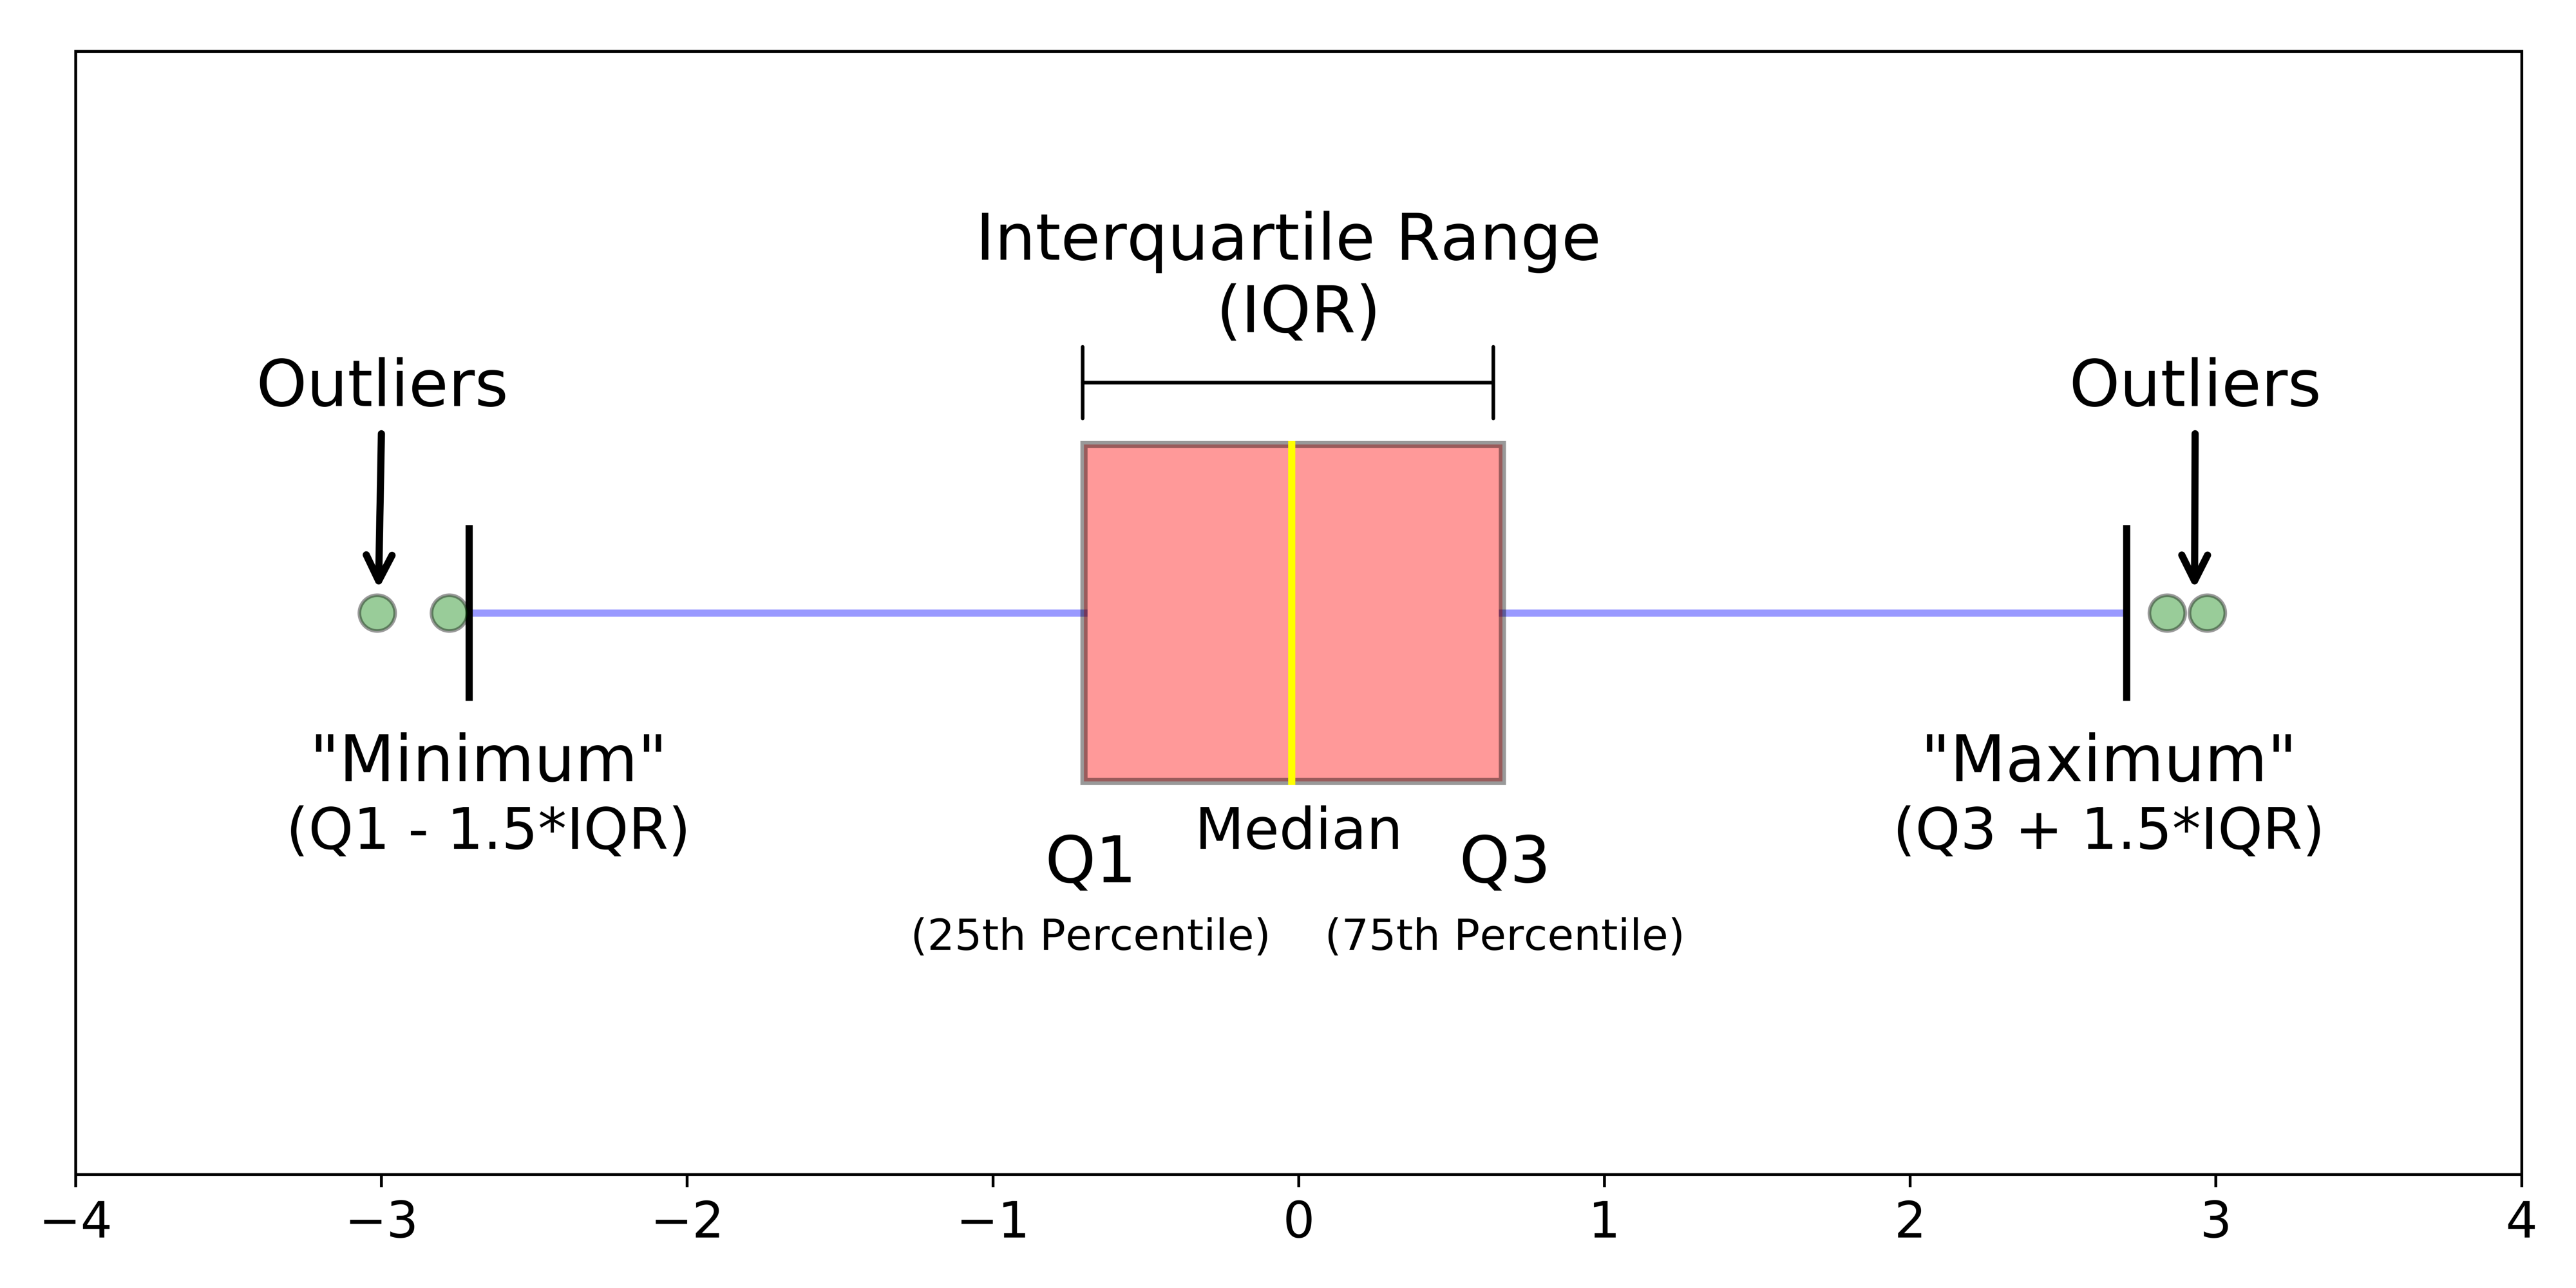
\includegraphics[scale=0.1]{1_2c21SkzJMf3frPXPAR_gZA}
Em que Minimum representa a barreira inferior, $ BI = Q_1 - 1.5 \times (Q_3 - Q_1
)$ e Maximum representa a barreira superior,  $BS = Q_3 + 1.5 \times (Q_3 - Q_1
)$

\section{Teorema do limite central (T.L.C.)}
Este teorema afirma que quando o tamanho da amostra aumenta, a distribuição amostral da sua média aproxima-se cada vez mais de uma distribuição normal. O TLC permite afirmar que, para n suficientemente grande, se
verifica:
$$
P\left(\sqrt{n}\frac{\bar{X}-\mu}{\sigma}\leq z\right)\approx \Phi(z)
$$
Isto é, a distribuição (desconhecida) de $\bar{X}$ pode ser aproximada
pela distribuição $N(\mu, \sigma/\sqrt{n})$.
Analogamente:
$$
P\left(\frac{S_n-n\mu}{\sigma\sqrt{n}}\leq z\right)\approx \Phi(z)
$$
A aproximaç\~ao é considerada razoável para
n > 30.

\subsection{TLC em distribuiç\~ao Binomial}
Se $X \cap B(n, p)$, a v.a. $X$ pode ser considerada como sendo a
soma de $n$ variáveis aleatórias i.i.d. com distribuição $B(1, p)$. Para $n$ suficientemente grande tem-se:
$$
P\left(\frac{X-np}{\sqrt{np(1-p)}}\leq z\right) \approx \Phi(z)
$$
i.e., a distribuição binomial $B(n, p)$ da v.a. $X$ pode ser
aproximada pela distribuição normal $N(np,
\sqrt{np(1 - p)})$.
A aproximação é considerada satisfatória
quando $np > 10$ e $n(1 - p) > 10$.

\subsection{TLC em distribuiç\~ao de Poisson}
Se $X \cap P(\lambda)$, a v.a. $X$ pode ser considerada como sendo a
soma de $n$ variáveis aleatórias i.i.d. com distribuição $P(\lambda/n)$. 
Para $\lambda$ suficientemente grande tem-se:
$$
P\left(\frac{X-\lambda}{\sqrt{\lambda}} \leq z \right) \approx \Phi(z)
$$
i.e., a distribuição de Poisson $P(\lambda)$ da v.a. $X$ pode ser
aproximada pela distribuição normal $N(\lambda, \sqrt{\lambda})$.
A aproximação considera-se satisfatória para
$\lambda > 20$.

\section{Testes de Hipóteses e Intervalos de confiança}
\begin{itemize}
\item[z] A forma $z_x$ representa a tabela da normal (parte final) com o valor $x$
\item[t] A forma $t_{x;y}$ representa a tabela da t de student, linha $x$ coluna $y$
\item[\^p] Recolhida uma amostra de dimensão n da população, seja X o
número de elementos da amostra que pertencem a uma dada categoria. \^p representa a proporção de elementos de uma amostra que pertencem a essa categoria. $$\hat{p} = \frac{X}{n}$$
\item[m/n/M/N] Número de elementos da amostra / população
\item[S/$\sigma$] Desvio padr\~ao da amostra / população
\item[$S^2 / \sigma^2$] Variância da amostra / população
\item[$\bar{X}$/$\mu$] Média da amostra / população
\end{itemize}
\end{document}